% !TEX program = xelatex
% A0 portrait poster -- petrol + copper palette, sections with subsections.
% Compile with XeLaTeX or LuaLaTeX:  latexmk -xelatex poster_portrait.tex
\documentclass{article}
\usepackage[paperwidth=84.1cm,paperheight=118.9cm,
            left=2.2cm,right=2.2cm,top=10.5cm,bottom=2.2cm]{geometry}
\usepackage{fontspec}
\usepackage{amsmath,amssymb}
\usepackage{xcolor}
\usepackage{tikz}
\usetikzlibrary{calc}
\usepackage[most]{tcolorbox}
\usepackage{enumitem}
\usepackage{microtype}
\usepackage{graphicx}

\IfFontExistsTF{Arial}{\setmainfont{Arial}}{\setmainfont{Liberation Sans}}
\pagestyle{empty}
\setlength{\parindent}{0pt}
\setlength{\parskip}{0.38em}
\setlist[itemize]{leftmargin=1.1em,itemsep=0.18em,topsep=0.25em,parsep=0pt}

% ---------------------------------------------------------------- palette
\definecolor{Petrol}{HTML}{123B4A}      % header, section bars
\definecolor{PetrolDeep}{HTML}{0C2A35}  % take-home band
\definecolor{Copper}{HTML}{D0703C}      % single accent
\definecolor{CopperPale}{HTML}{FBEDE4}  % claim background
\definecolor{PetrolPale}{HTML}{E4EDEF}  % secondary highlight
\definecolor{Paper}{HTML}{F4F6F5}
\definecolor{Ink}{HTML}{1E2A30}
\definecolor{Mid}{HTML}{66747A}
\definecolor{Rule}{HTML}{CFD8DA}
\definecolor{Placeholder}{HTML}{E9EDEC}
% variable colours (kept distinct from the frame colours)
\definecolor{Ucol}{HTML}{C61826}  % activator
\definecolor{Vcol}{HTML}{0072B2}  % inhibitor
\definecolor{Rcol}{HTML}{7B4FA0}  % source density

\newcommand{\U}{\textcolor{Ucol}{u}}
\newcommand{\V}{\textcolor{Vcol}{v}}
\newcommand{\R}{\textcolor{Rcol}{\rho}}

\color{Ink}
\newcommand{\bodyfont}{\fontsize{22}{27.5}\selectfont}
\newcommand{\smallfont}{\fontsize{19}{23.5}\selectfont}
\newcommand{\tinyfont}{\fontsize{14}{17}\selectfont}
\newcommand{\eqnfont}{\fontsize{22}{28}\selectfont}
\newcommand{\placeholderfont}{\fontsize{19}{23}\selectfont\bfseries\color{Mid}}

% ---------------------------------------------------------------- layout
\newlength{\colw}\setlength{\colw}{38.6cm}
\newlength{\secgap}\setlength{\secgap}{0.8cm}

% full-width section bar
\newcommand{\postersection}[2]{%
  \par\noindent
  \begin{tikzpicture}
    \fill[Petrol,rounded corners=3mm] (0,0) rectangle (\linewidth,2.4cm);
    \node[anchor=west,text=white,font=\fontsize{36}{40}\selectfont\bfseries]
      at (1.0cm,1.2cm) {\textcolor{Copper}{#1}\hspace{0.7em}#2};
  \end{tikzpicture}\par\vspace{0.5cm}%
}

% subsection heading inside a column
\newcommand{\postersub}[2]{%
  \par\vspace{0.4cm}\noindent
  {\fontsize{27}{31}\selectfont\bfseries\color{Copper}#1\hspace{0.45em}\color{Petrol}#2}\par
  \vspace{-0.2cm}\noindent{\color{Copper}\rule{\linewidth}{1.6pt}}\par\vspace{0.1cm}%
}

\newcommand{\placeholder}[2]{%
  \par\noindent
  \begin{tikzpicture}
    \node[draw=Mid,dashed,line width=1.4pt,rounded corners=3mm,fill=Placeholder,
          minimum width=\linewidth,minimum height=#1,text width=0.85\linewidth,
          align=center,inner sep=0pt] {\placeholderfont #2};
  \end{tikzpicture}\par
}

\newcommand{\claim}[1]{%
  \begin{tcolorbox}[enhanced,colback=CopperPale,colframe=Copper,boxrule=1.4pt,arc=3mm,
                    left=7mm,right=7mm,top=4mm,bottom=4mm,before skip=0.3cm,after skip=0.1cm]
  \centering\fontsize{26}{32}\selectfont\bfseries\color{Petrol}#1\par
  \end{tcolorbox}%
}

\newcommand{\note}[1]{%
  \begin{tcolorbox}[colback=PetrolPale,colframe=PetrolPale,boxrule=0pt,arc=2mm,
                    left=5mm,right=5mm,top=3mm,bottom=3mm,before skip=0.4cm,after skip=0.2cm]
  \fontsize{20}{25}\selectfont\bfseries\color{Petrol}#1
  \end{tcolorbox}%
}

\newcommand{\minitag}[1]{\tikz[baseline=(X.base)]\node[fill=PetrolPale,rounded corners=2mm,
    inner xsep=3mm,inner ysep=1.5mm,text=Petrol,font=\fontsize{17}{19}\selectfont\bfseries] (X) {#1};}

\newsavebox{\colboxL}\newsavebox{\colboxR}\newlength{\colH}
% balanced columns: both columns get the height of the taller one; \vfill stretches
\newcommand{\balcols}[2]{%
  \sbox{\colboxL}{\begin{minipage}[t]{\colw}\bodyfont #1\end{minipage}}%
  \sbox{\colboxR}{\begin{minipage}[t]{\colw}\bodyfont #2\end{minipage}}%
  \colH=\dimexpr\ht\colboxL+\dp\colboxL\relax
  \ifdim\dimexpr\ht\colboxR+\dp\colboxR\relax>\colH \colH=\dimexpr\ht\colboxR+\dp\colboxR\relax\fi
  \begin{minipage}[t][\colH][s]{\colw}\bodyfont #1\par\vspace{0pt}\end{minipage}\hfill
  \begin{minipage}[t][\colH][s]{\colw}\bodyfont #2\par\vspace{0pt}\end{minipage}\par}
\newenvironment{leftcol}{\begin{minipage}[t]{\colw}\bodyfont}{\end{minipage}\hfill}
\newenvironment{rightcol}{\begin{minipage}[t]{\colw}\bodyfont}{\end{minipage}}

% ================================================================ document
\begin{document}
\pagecolor{Paper}
\begin{tikzpicture}[remember picture,overlay]
  \fill[Paper] (current page.south west) rectangle (current page.north east);
  % header
  \fill[Petrol] (current page.north west) rectangle ([yshift=-9.0cm]current page.north east);
  \fill[Copper] ([yshift=-9.0cm]current page.north west) rectangle ([yshift=-9.4cm]current page.north east);
  \node[anchor=north west,inner sep=0pt,text width=66cm,text=white,
        align=left,font=\fontsize{50}{58}\selectfont\bfseries] (title)
    at ([xshift=2.2cm,yshift=-2.3cm]current page.north west)
    {Pattern Formation and Positional Memory in Hydra Regeneration Models};
  \node[anchor=north west,inner sep=0pt,text width=57cm,text=white,
        font=\fontsize{25}{31}\selectfont] (authors)
    at ([yshift=-0.9cm]title.south west)
    {Szymon~Cygan \quad\textperiodcentered\quad Anna~Marciniak-Czochra
     \quad\textperiodcentered\quad Finn~Münnich \quad\textperiodcentered\quad Moritz~Mercker};
  \node[anchor=north west,inner sep=0pt,text width=57cm,text=white!75!Petrol,
        font=\fontsize{20}{25}\selectfont]
    at ([yshift=-0.35cm]authors.south west)
    {Heidelberg University, Heidelberg, Germany};
  % logo: white-text version straight on the petrol header
  % (alternative: original logo on a white plate ->
  %  \node[...,fill=white,rounded corners=4mm,inner sep=6mm]{
\includegraphics[height=5cm]{assets/heidelberg_logo.png}};)
  \node[anchor=north east,inner sep=0pt]
    at ([xshift=-2.2cm,yshift=-1.5cm]current page.north east)
    {
\includegraphics[height=6.0cm]{assets/heidelberg_logo_white.png}};
\end{tikzpicture}%
\noindent
% ================================================================ 1
\postersection{1}{Motivation}
\begin{leftcol}
  \postersub{1.1}{Hydra as a patterning problem}
  \begin{minipage}[t]{25.0cm}\vspace{0pt}
    \centering
    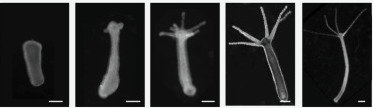
\includegraphics[height=7.2cm]{assets/steichele2024_control_regeneration_paper.png}\par
    \vspace{0.08cm}
    {\tinyfont\color{Mid}Control: a headless fragment regenerates a complete head.\\
    Steichele, M. \emph{et al.} (2024). \emph{Life Sci. Alliance} 7, e202403054.\par}
  \end{minipage}\hfill
  \begin{minipage}[t]{11.0cm}\vspace{0pt}
    \centering
    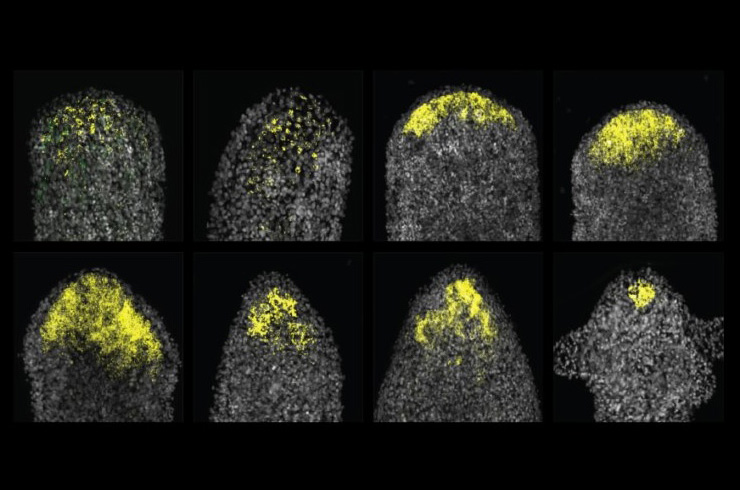
\includegraphics[height=7.2cm]{assets/nuninger2026_wnt3_regeneration.jpg}\par
    \vspace{0.10cm}
    {\tinyfont\color{Mid}Wnt3 focuses at the future head organiser.\\
    Nuninger, J. \emph{et al.} (2026). \emph{Nat. Commun.}\par}
  \end{minipage}
\end{leftcol}
\begin{rightcol}
  % introduction (no subsection header), aligned with the images of 1.1
  \vspace{2.3cm}
  {\raggedright \emph{Hydra} regenerates a head after amputation, forms a single head,
  and remembers the original polarity of its tissue. Each head is built around a head
  organiser marked by Wnt/$\beta$-catenin signalling: during regeneration, Wnt3 becomes
  localised at the tip of the future head. Behind this behaviour lie three different
  phenomena:\par}
  \begin{itemize}[itemsep=0.2em,topsep=0.4em]
    \item regeneration,
    \item pattern selection,
    \item positional memory.
  \end{itemize}
  {\raggedright Activator--inhibitor models already explain regeneration and pattern selection,
  but positional memory requires an additional variable: source density.\par}
\end{rightcol}


\vspace{\secgap}
% ================================================================ 2
\postersection{2}{What the activator--inhibitor model already does}
\balcols{%
  \postersub{2.1}{Production terms change the phase portrait}
  {\fontsize{28}{36}\selectfont
  \[
  \begin{aligned}
  \partial_t \U &= D_u\Delta \U + \frac{a \U^2+q_u}{\V}-\mu_u \U+p_u,\\
  \partial_t \V &= D_v\Delta \V + b \U^2-\mu_v \V+p_v,
  \end{aligned}
  \qquad x\in[0,L],\ t\geqslant 0
  \]\par}
  \vspace{0.5cm}
  \begin{minipage}[t]{17.6cm}\vspace{0pt}\smallfont\raggedright
  \begin{itemize}[topsep=0pt]
    \item $\U$: activator, short-range and self-enhancing,
    \item $\V$: inhibitor, long-range, produced by $u$.
  \end{itemize}
  \end{minipage}\hfill
  {\color{Rule}\vrule width 1.5pt}\hfill
  \begin{minipage}[t]{19.6cm}\vspace{0pt}\smallfont
  \begin{itemize}[topsep=0pt]
    \item $p_v$: basal inhibitor production,
    \item $p_u$: external activator input,
    \item $q_u$: activator input under inhibitor regulation.
  \end{itemize}
  \end{minipage}
  \par\vspace{0.35cm}
  {\smallfont\textbf{\color{Petrol}Nullclines}\par}
  \vspace{0.1cm}
  {\fontsize{17}{21}\selectfont
  \tikz[baseline=-0.6ex]\draw[Ucol,line width=2.5pt](0,0)--(0.9,0); $u$-nullcline\quad
  \tikz[baseline=-0.6ex]\draw[Vcol,line width=2.5pt](0,0)--(0.9,0); $v$-nullcline\quad
  \tikz[baseline=-0.6ex]\fill[Petrol](0,0) circle (0.22); stable rest\quad
  \tikz[baseline=-0.6ex]\draw[Copper,line width=2.5pt,fill=Paper](0,0) circle (0.2); unstable threshold\quad
  \tikz[baseline=-0.6ex]\fill[Copper](0,0) circle (0.22); active state (Turing candidate)\par}
  \vspace{0.3cm}
  \begin{minipage}[t]{18.8cm}\vspace{0pt}
    {\centering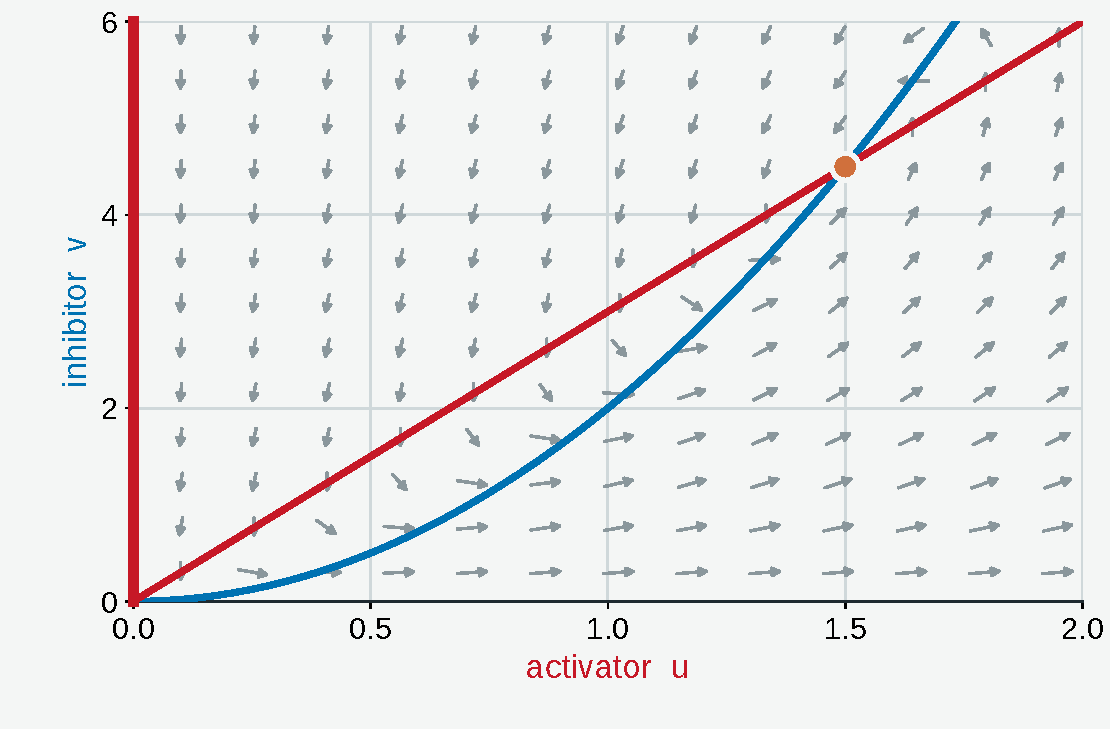
\includegraphics[width=12cm]{generated/phase_one_state.pdf}\par}
    \smallfont\centering
    \textbf{1 steady state} ($p_v=p_u=q_u=0$)\\
    no resting state: an arbitrary perturbation leads to a pattern.
  \end{minipage}\hfill
  \begin{minipage}[t]{18.8cm}\vspace{0pt}
    {\centering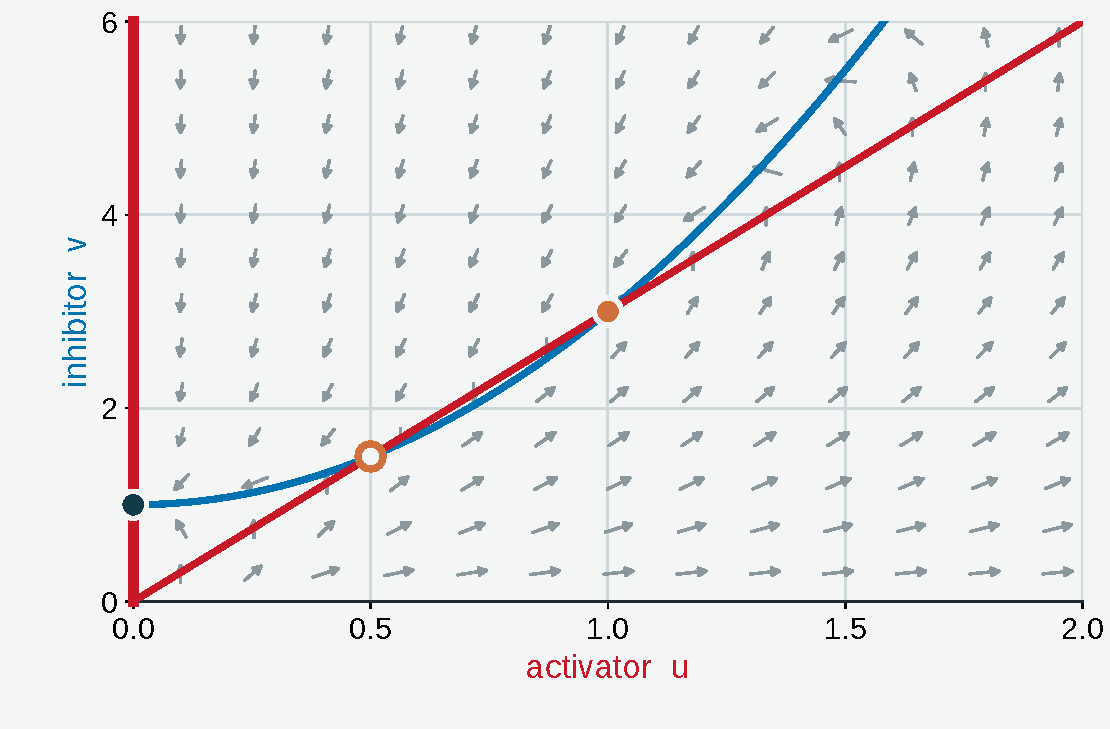
\includegraphics[width=12cm]{generated/phase_three_states.pdf}\par}
    \smallfont\centering
    \textbf{3 steady states} ($p_v>0$)\\
    small perturbations vanish back to the rest state $u=0$.
  \end{minipage}

  \vspace{0.8cm}\vfill
  \postersub{2.2}{Inhibitor production is essential}
  \begin{minipage}[t]{18.6cm}\vspace{0pt}\smallfont\raggedright
  \textbf{\color{Petrol}$p_v=0$:}\   Only one steady state, which can be Turing unstable.
  Any perturbation forms a pattern.
  \end{minipage}\hfill
  {\color{Rule}\vrule width 1.5pt}\hfill
  \begin{minipage}[t]{18.6cm}\vspace{0pt}\smallfont\raggedright
  \textbf{\color{Petrol}$p_v>0$:}\   A stable rest state, an activation threshold
  and a pattern-forming state.
  \end{minipage}\par
  \note{For everything that follows it is essential to have more than one
  steady state.}
}{%
  \postersub{2.3}{Pattern selection depends on history}
  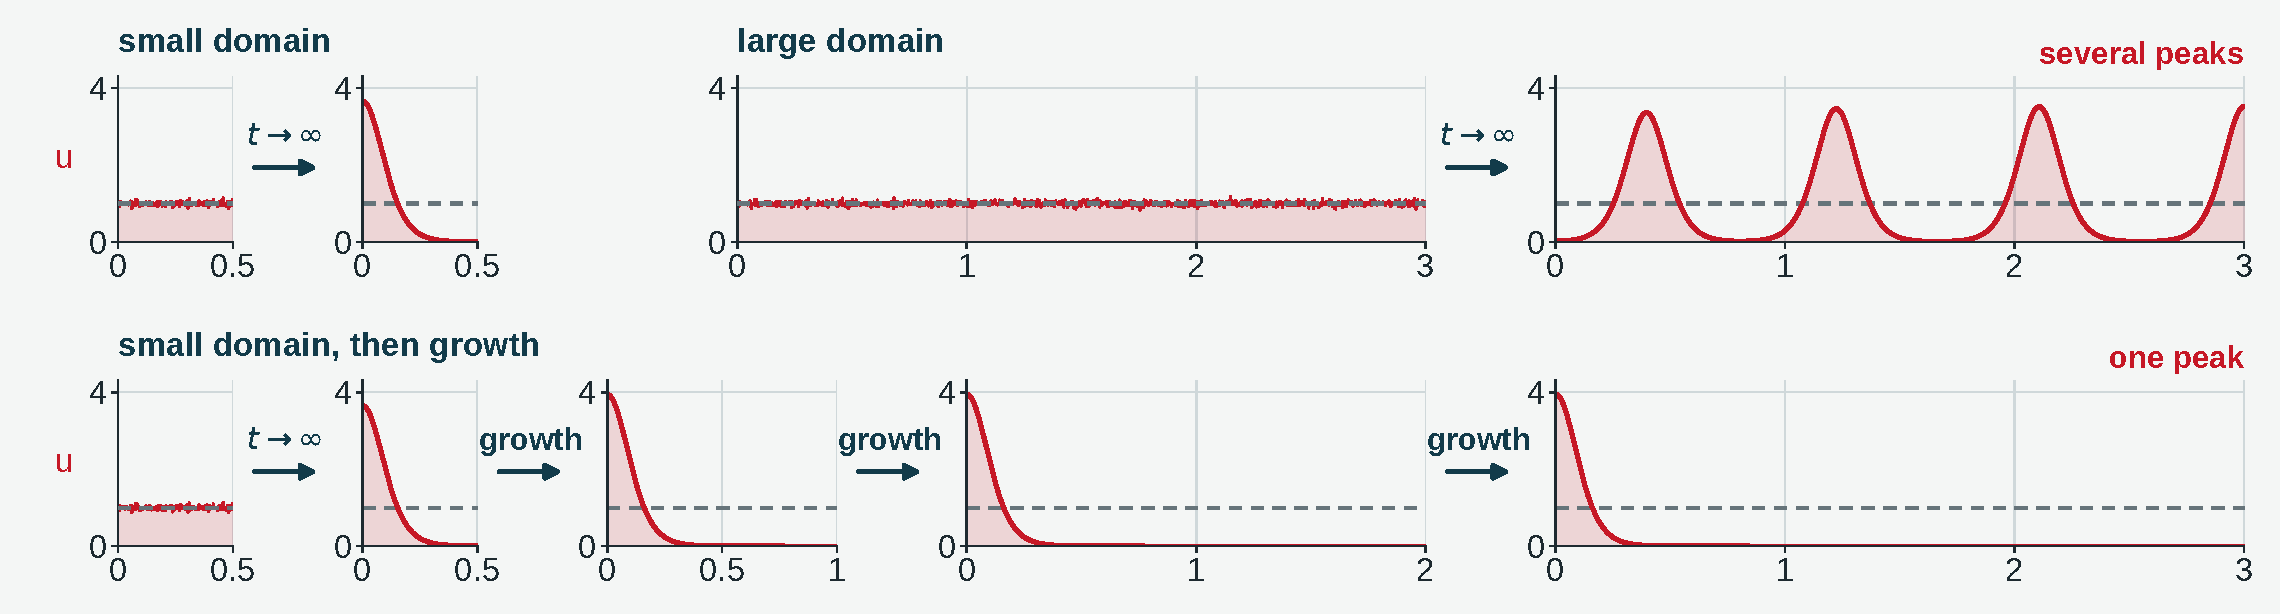
\includegraphics[width=\linewidth]{generated/pattern_history.pdf}\par
  \vspace{0.2cm}
  \smallfont
  Starting near the diffusion-unstable state $E_+$, a small domain forms one peak
  and a large domain several. Growing the small domain to the same large size
  keeps a single peak.

  \vspace{0.8cm}\vfill
  \postersub{2.4}{Regeneration needs a wound}
  \smallfont
  Removing the head by cutting triggers regeneration.
  Removing it by ligation, without a wound, does not.\par
  \vspace{0.3cm}
  \begin{minipage}[c]{15.0cm}
    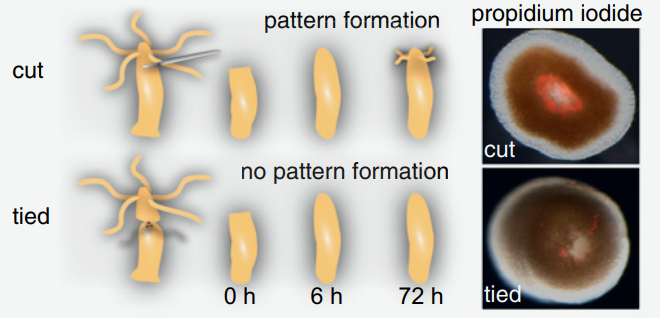
\includegraphics[width=\linewidth]{assets/tursch_cut_tied_paper.png}\par
    {\centering\tinyfont\color{Mid} Tursch et al., \textit{PNAS} 119 (2022), Fig.~1A.\par}
  \end{minipage}\hfill
  \begin{minipage}[c]{23.0cm}
    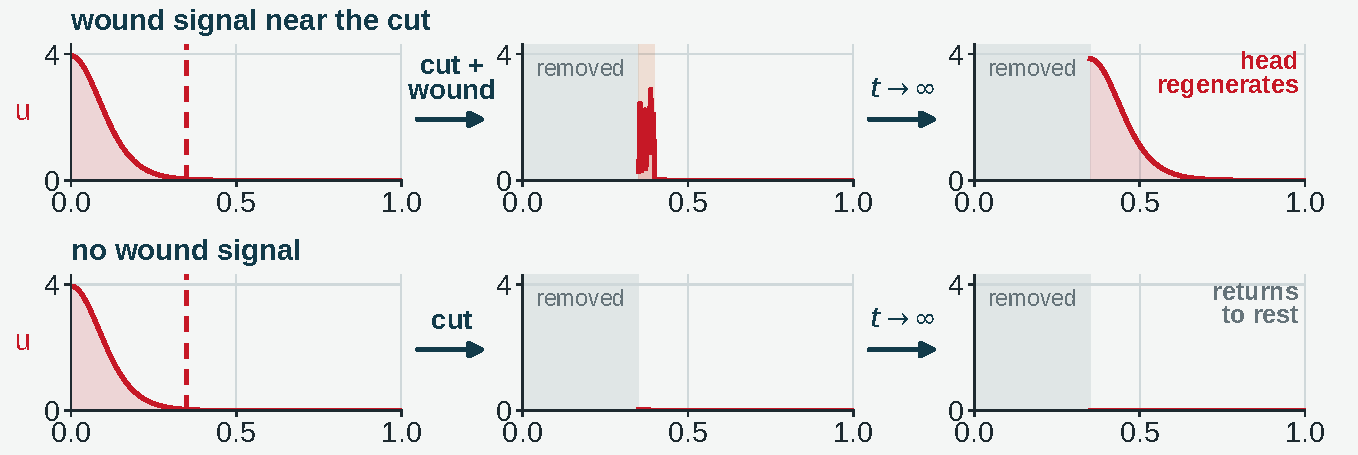
\includegraphics[width=\linewidth]{generated/regeneration_sims.pdf}
  \end{minipage}\par
  \vspace{0.3cm}
  \smallfont
  Bistability is essential. With a single steady state regeneration always
  occurs. With three steady states the system is bistable, the cut tissue returns
  to rest and only a large perturbation from the wound brings back a pattern.
  Biologically, this perturbation is the wound response. Injury triggers
  Ca$^{2+}$ and ROS signalling, which activates MAPKs and up-regulates Wnt3
  at every cut, independent of its position (Tursch et al., 2022).\par

}

\vspace{0.8cm}
\postersub{2.5}{Grafts - the model chooses the position}
\vspace{0.4cm}
\begin{minipage}[c]{\colw}
  \centering
  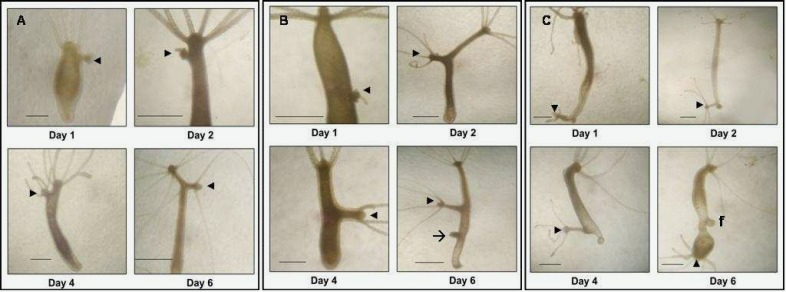
\includegraphics[width=26.5cm]{assets/kadu2012_grafting_paper.png}\par
  \vspace{0.1cm}
  {\tinyfont\color{Mid}Kadu, V., Ghaskadbi, S.~S. \& Ghaskadbi, S. (2012).
  Int. J. Mol. Cell. Med. 1(1), 11--20. CC BY 3.0.\par}
\end{minipage}\hfill
\begin{minipage}[c]{\colw}
  \centering
  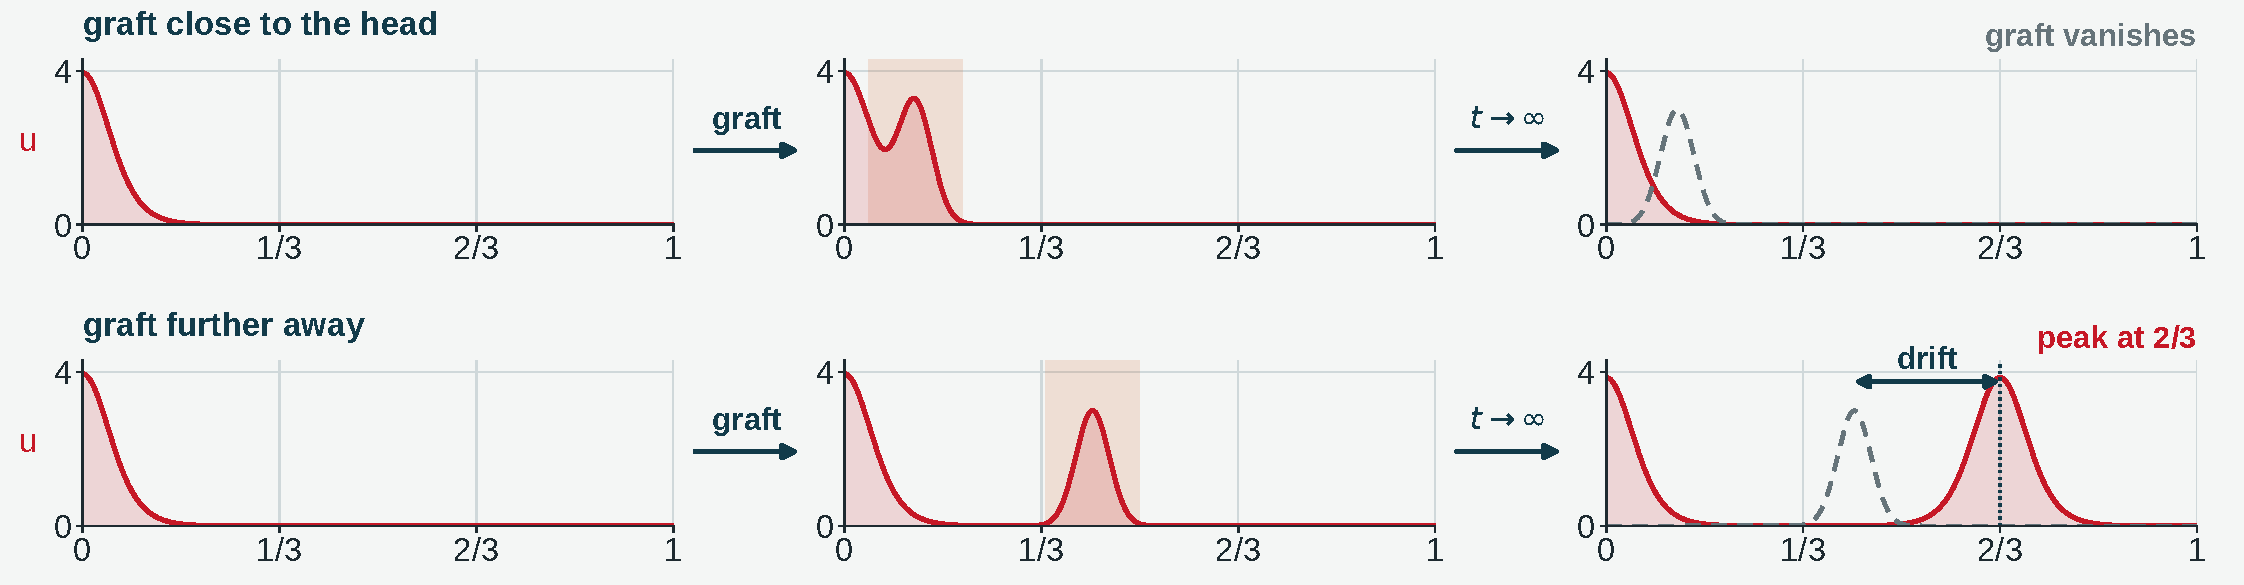
\includegraphics[width=38.0cm]{generated/graft_drift.pdf}
\end{minipage}\par

% \claim{Source density is not needed to make a head --- but the model, not the wound, decides where the head ends up.}

\vspace{\secgap}
% ================================================================ 3
\postersection{3}{Positional memory and source density}
\begin{leftcol}
  \postersub{3.1}{Grafting exposes missing information}
  {\centering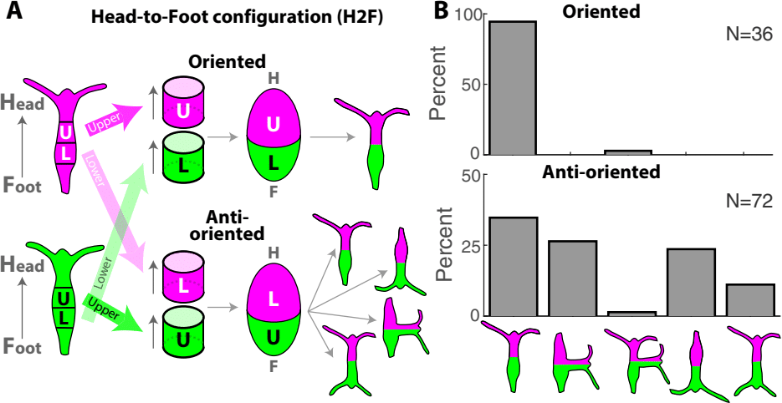
\includegraphics[width=0.78\linewidth]{assets/livshits_h2f_experiment_transparent.png}\par}
  {\tinyfont\color{Mid} Head-to-foot grafts, oriented vs.\ anti-oriented. Livshits et al.\ (2022), K.~Keren group.\par}
  \smallfont
  Reversing the orientation of comparable tissue pieces changes the
  distribution of outcomes. Near the resting state, \U\ and \V\ alone do not
  distinguish an upper-body fragment from a lower-body one.

  \vspace{0.6cm}
  \postersub{3.2}{Prescribed $\rho(x)$ as tissue competence}
  \begin{minipage}[c]{20.8cm}
    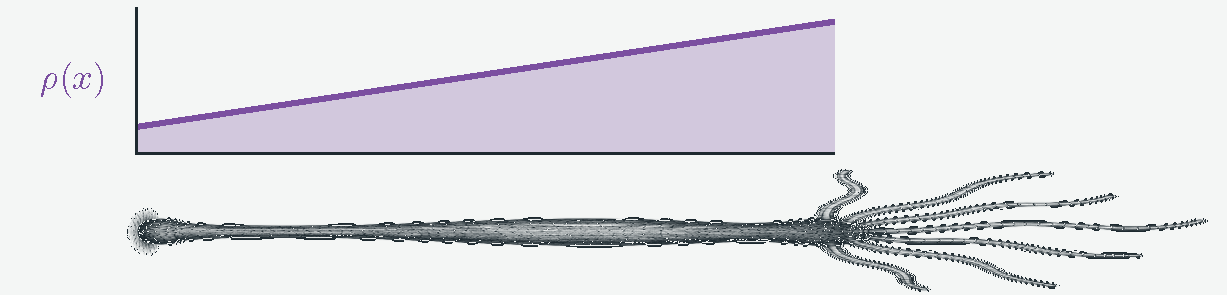
\includegraphics[width=20.77cm]{generated/hydra_rho.pdf}
  \end{minipage}\hfill
  \begin{minipage}[c]{17.3cm}\fontsize{28}{36}\selectfont
  \[
  \begin{aligned}
  \partial_t \U &= D_u\Delta \U + \R(x)\,\frac{a \U^2}{\V} - \mu_u \U,\\
  \partial_t \V &= D_v\Delta \V + \R(x)\, b \U^2 - \mu_v \V + p_v.
  \end{aligned}
  \]
  \end{minipage}\par
  \vspace{0.3cm}
  {\centering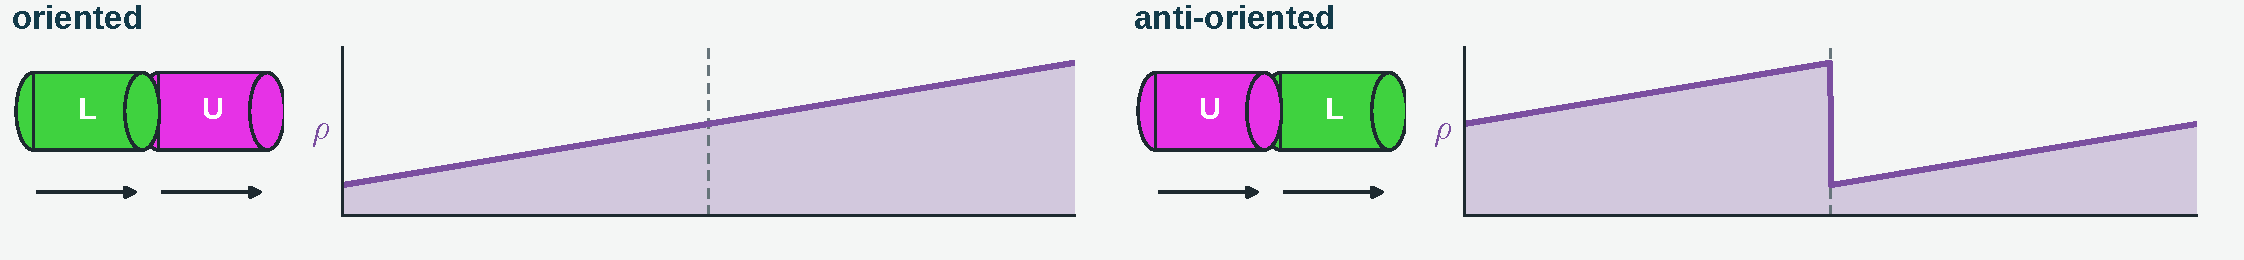
\includegraphics[width=\linewidth]{generated/rho_profiles.pdf}\par}
  \vspace{0.2cm}
  \smallfont
  A fixed source-density profile encodes tissue origin before the activator
  is present and biases where a wound-triggered peak forms (source-gradient
  idea, Suzuki \& Takagi 2011).
\end{leftcol}
\begin{rightcol}
  \postersub{3.3}{Dynamic source density model}
  \begin{minipage}[c]{20.5cm}\fontsize{28}{36}\selectfont
  \[
  \begin{aligned}
  \partial_t \U &=D_u\Delta \U+\R\,\frac{a \U^2}{\V}-\mu_u \U,\\
  \partial_t \V &=D_v\Delta \V+b\R\,\U^2-\mu_v \V+p_v,\\
  \tau\,\partial_t\R&=D_\rho\Delta\R+\U-\R.
  \end{aligned}
  \]
  \end{minipage}\hfill
  {\color{Rule}\vrule width 1.5pt}\hfill
  \begin{minipage}[c]{16.8cm}\smallfont\raggedright
  \begin{itemize}[topsep=0pt]
    \item $\rho(0,x)$ stores the grafted configuration,
    \item $\tau$ sets the lifetime of memory,
    \item $D_\rho$ communicates positional information in space.
  \end{itemize}
  \end{minipage}\par
  \vspace{0.0cm}
  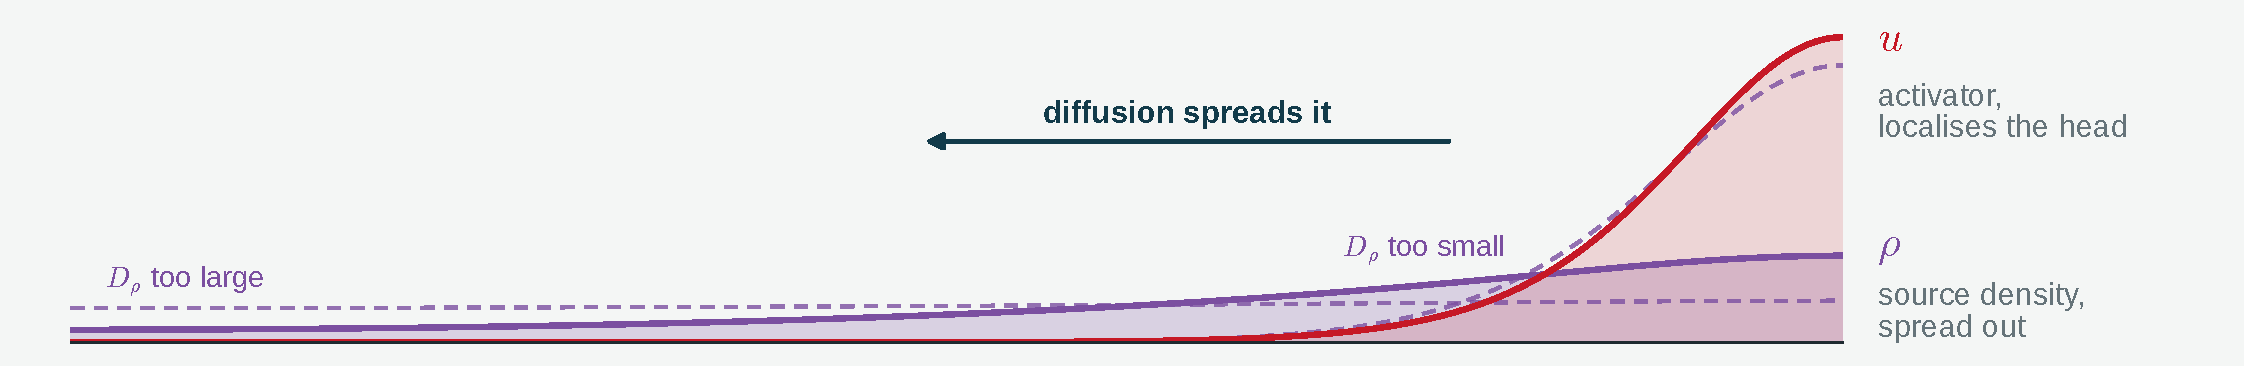
\includegraphics[width=\linewidth]{generated/rho_diffusion.pdf}\par
  \vspace{0.2cm}
  \smallfont
  $D_\rho$ too small: memory stays sharply localised. Intermediate: a usable
  gradient forms. Too large: spatial information is erased.

  \vspace{0.6cm}
  \postersub{3.4}{Static vs dynamic source density - metastability of patterns} 
  \smallfont Three tissue pieces generate a piecewise-linear initial source-density profile. Wounds are induced at the two graft interfaces.

  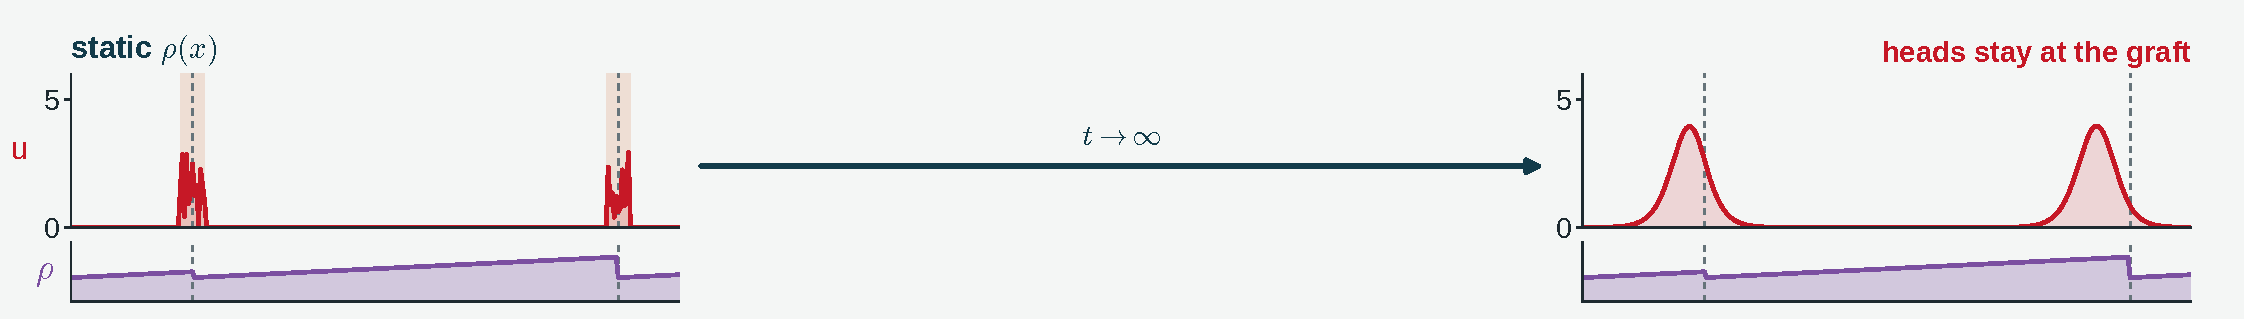
\includegraphics[width=\linewidth]{generated/rho_static.pdf}\par
  \vspace{0.2cm}
  \smallfont Static source density $ \rho(x) $: activator peaks form near the wound sites and remain there. These positions are not Turing-selected, but the two-peak state is stable and may mark sites of new-axis formation.
  
  \vspace{0.2cm}
  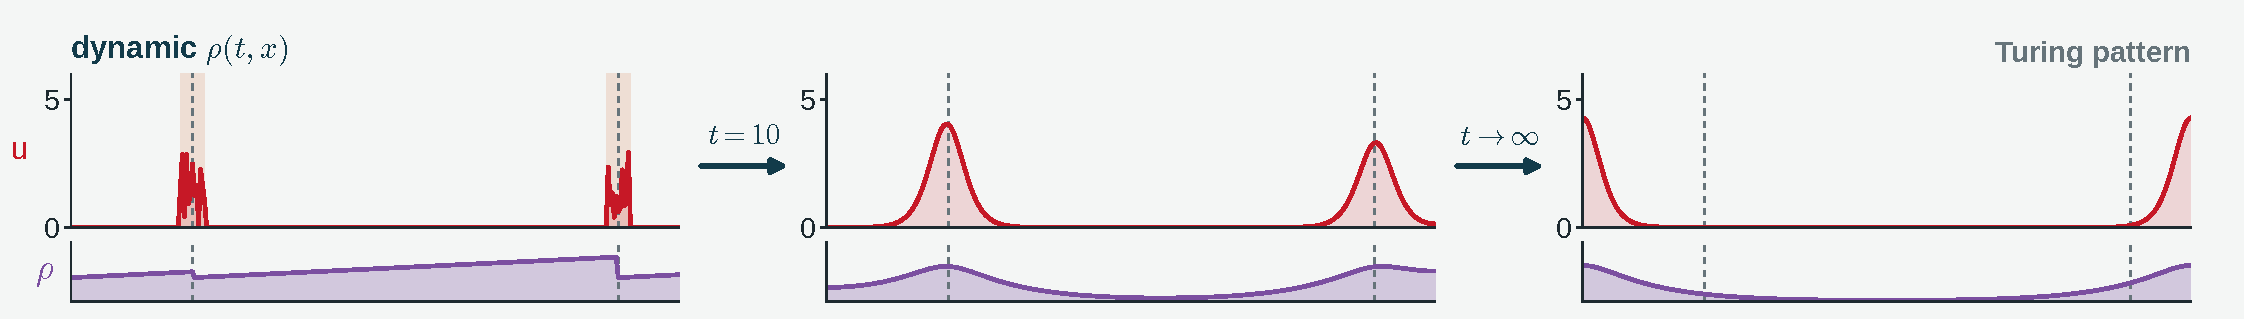
\includegraphics[width=\linewidth]{generated/rho_dynamic.pdf}\par
  \vspace{0.2cm}
  \smallfont
  The source density is initialised as $ \rho(x,0)=\rho_0(x) $, with large $ \tau $ chosen so that its dynamics is slow relative to $ u $ and $ v $. On the fast activator-inhibitor timescale, peaks form near the graft interfaces as in the static case. This graft-pinned configuration is metastable and, as $ \rho $ relaxes, eventually destabilises towards the Turing-selected two-head pattern.
\end{rightcol}

% \claim{Source density can hold positional memory for a long time --- without making the graft-selected peak truly stationary.}

\vfill
% ================================================================ 4
\begin{tcolorbox}[enhanced,colback=PetrolDeep,colframe=PetrolDeep,arc=3mm,
                  left=1.0cm,right=1.0cm,top=0.7cm,bottom=0.7cm,before skip=0pt,
                  fontupper=\fontsize{30}{36}\selectfont\bfseries\color{white}]
\centering Source density is not needed to make a head.
\textcolor{Copper}{It may be needed to remember where a head should form.}
\end{tcolorbox}
\end{document}
